\documentclass{beamer}

\usepackage{graphicx}
\usepackage[latin1]{inputenc}
\usepackage[T1]{fontenc}
\usepackage[english]{babel}
\usepackage{listings}
\usepackage{xcolor}
\usepackage{eso-pic}
\usepackage{mathrsfs}
\usepackage{url}
\usepackage{amssymb}
\usepackage{amsmath}
\usepackage{multirow}
\usepackage{booktabs}
\usepackage{hyperref}
\usepackage{booktabs}
\usepackage{bbm}
\usepackage{cooltooltips}
\usepackage{colordef}
\usepackage{beamerdefs}
\usepackage{lvblisting}
\usepackage{color}

\pgfdeclareimage[height=3.5cm]{logobig}{hucaselogo}
\pgfdeclareimage[height=0.7cm]{logosmall}{Figures/LOB_Logo}

\renewcommand{\titlescale}{1.0}
\renewcommand{\titlescale}{1.0}
\renewcommand{\leftcol}{0.6}

\title[DCC Garch Model]{DCC Garch Model}
\authora{Yinan Wu}
\authorb{}
\authorc{}

\def\linka{http://lvb.wiwi.hu-berlin.de}
\def\linkb{http://case.hu-berlin.de}
\def\linkc{}

\institute{Ladislaus von Bortkiewicz Chair of Statistics \\
C.A.S.E. -- Center for Applied Statistics\\
and Economics\\
Humboldt--Universit\"at zu Berlin \\}

\hypersetup{pdfpagemode=FullScreen}

\begin{document}
\frame[plain]{
\titlepage
}
\section{Introduction}
{
\frame{
\frametitle{Background}
\begin{itemize}
\item{Volatility varies over time and tends to cluster in periods - heteroscedatisity.}
\item{Volatility has shown to be autocorrelated.}

\end{itemize}

}


\frame{
\frametitle{What is DCC Garch Model}
\begin{itemize}
\item{The dynamic conditional correlations proposed by Engle and Tse and Tsui(2002).}
\item{It can be estimated in two steps to make the model relatively easy to use in practice.}

\end{itemize}
\smallskip
The two steps:\\
\begin{enumerate}
\item{The conditional variance is estimated via unvariate GARCH model for respectively asset.}
\item{The parameters for the conditional correlation given the parameters from the first step
are estimated.}
\end{enumerate}

}
{
\frame{
\frametitle{GARCH Model Estimation}
\begin{itemize}
\item{The simplest and popular GARCH model is the GARCH(1,1)}
\end{itemize}
\begin{center}

$h_t=\omega+\delta \eta_{t-1}^2+\gamma h_{t-1}$\\
\bigskip
\bigskip

where $ \omega>=0, \delta>=0, \gamma>=0$
\end{center}
}

\frame{
\frametitle{DCC Model Estimation}

\begin{itemize}
\item{In the DCC model, the covariance matrix is decomposed into}
\end{itemize}
\begin{center}
$H_t=D_tR_tD_t$
\end{center}
\bigskip
Remarks:\\
$D_t$ is a diagonal matrix of time varying standard variation from univariate GARCH - processes.\\
$R_t$ is the conditional correlation matrix of the standardized disturbances $\varepsilon_t$.\\

}
}

\section{Example}
\frame{
\frametitle{The DCC-model in Practice}
\begin{itemize}
\item{Portfolio: four stocks consisting Apple, Google, Nike and Microsoft obtained from Yahoo Finance.}
\item{Time Period: From 2009-12-14 to 2012-12-12 daily data, 755 observations.}
\item{The initial value is 10000 US-Dollar.}
\item{The estimation window is 734, and The rolling window is 20 days.}
\item{The log return was assumed to be normally distributed.}
\end{itemize}
}

\frame{
\frametitle{Not Normally Distributed}
\begin{center}
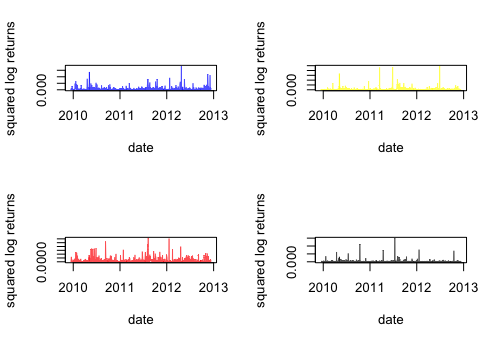
\includegraphics[scale=0.45]{gp11}\\
\smallskip
\small{Figure 1. Squared returns on daily data from December 2009 to December 2012.}
\end{center}
}
\frame{
\frametitle{Time Series Data of Log Return}
\begin{center}
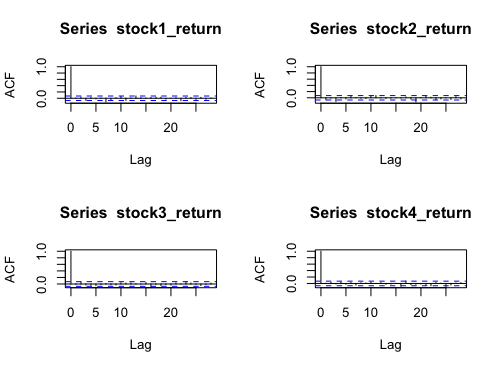
\includegraphics[scale=0.40]{gp21}\\
\smallskip
\small{Figure 2. ACF of returns on daily data from December 2009 to December 2012.}
\end{center}
}
\frame{
\frametitle{Time Series Data of Log Return Cont.}
\begin{center}
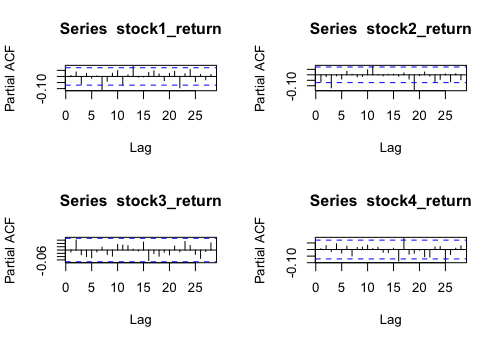
\includegraphics[scale=0.45]{gp22}\\
\smallskip
\small{Figure 3. PACF of returns on daily data from December 2009 to December 2012.}
\end{center}
}

\frame{
\frametitle{Estimation Model}
\begin{itemize}
\item{Arma(1,0), Normally distributed, DCC (1,1) }
\item{Arma(1,0), Student t distributed, DCC (1,1) }
\item{Arma(1,0), Student t distributed, DCC (2,1) }
\end{itemize}

}
}



\section{Risk}
\frame{
\frametitle{VaR estimation Results}
\begin{center}
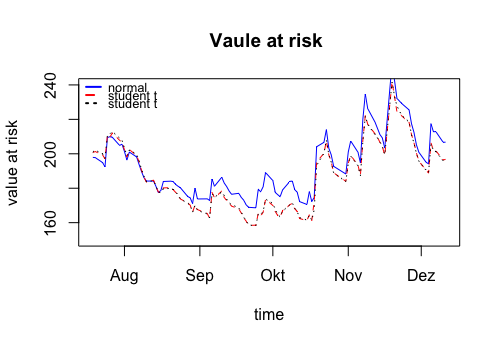
\includegraphics[scale=0.45]{gp3}\\
\smallskip
\small{Figure 4. 100 days Value at Risk estimation.}
\end{center}

}
{\frame{
\frametitle{Value at Risk 95\% for 20 days forecasting }
\begin{center}
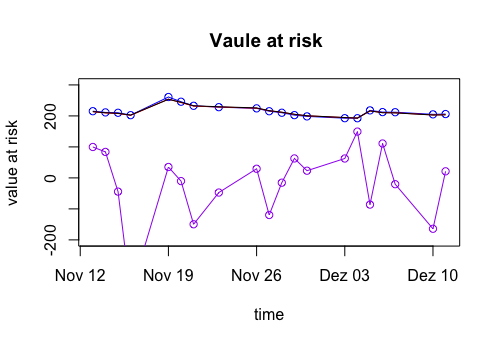
\includegraphics[scale=0.45]{gp4}\\
\smallskip
\small{Figure 5. 20 day forecasting of value at risk and real loss.}
\end{center}
}

}
{\frame{
\frametitle{Value at Risk 95\% for 100 days forecasting}
\begin{center}
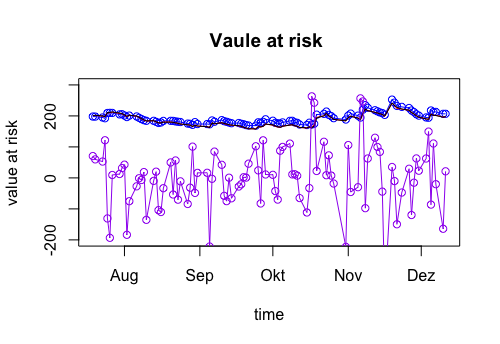
\includegraphics[scale=0.45]{gp55}\\
\smallskip
\small{Figure 6. 100 day forecasting of value at risk and real loss.}
\end{center}
}


}
\section{Conclusion}
{\frame{
\frametitle{Summary}
\begin{itemize}
\item{The DCC-model with suitably specified univariate GARCH-models is an appropriate model to use when 
forcasting the covariance matrix in the short run. }
\end{itemize}
}
}
\end{document}
